\noindent Configurada la herramienta, se podrán realizar análisis en el laboratorio construido utilizando Cuckoo Sandbox. Para ello, es necesario ejecutar una serie de comandos para iniciar correctamente el entorno cada vez que el sistema sea reiniciado:

\begin{enumerate}
\item En cada terminal que se abra para trabajar, iniciar el entorno virtual “cuckoo-test”: 
\begin{listing}[style=consola, numbers=none]
$ workon cuckoo-test 
\end{listing}
\item Activar forwarding para la interfaz de red:
\begin{listing}[style=consola, numbers=none]
(cuckoo-test) $ sudo sysctl -w net.ipv4.conf.wlo1.forwarding=1
\end{listing}
\item Crear interfaz con VMCloak:
\begin{listing}[style=consola, numbers=none]
(cuckoo-test) $ vmcloak-vboxnet0
\end{listing}
\item Ejecutar Cuckoo Rooter:
\begin{listing}[style=consola, numbers=none]
(cuckoo-test) $ cuckoo rooter --sudo --group gonzalo
\end{listing}
\item Ejecutar Cuckoo:
\begin{listing}[style=consola, numbers=none]
(cuckoo-test) $ cuckoo
\end{listing}
\item Ejecutar Cuckoo Web:
\begin{listing}[style=consola, numbers=none]
(cuckoo-test) $ cuckoo web --host 127.0.0.1 --port 8080
\end{listing}
\end{enumerate}

Una vez ejecutados estos comandos, si se accede en el navegador a la dirección 127.0.0.1:8080 se encontrará la página principal de la interfaz web de Cuckoo Sandbox, como muestra la Figura \ref{fig:DashboardCuckoo}, donde aparece información de la versión de la herramienta, detalles sobre el uso de memoria y otros. Además, desde aquí será posible subir una muestra para su análisis.


\begin{figure}[h!]
\begin{center}
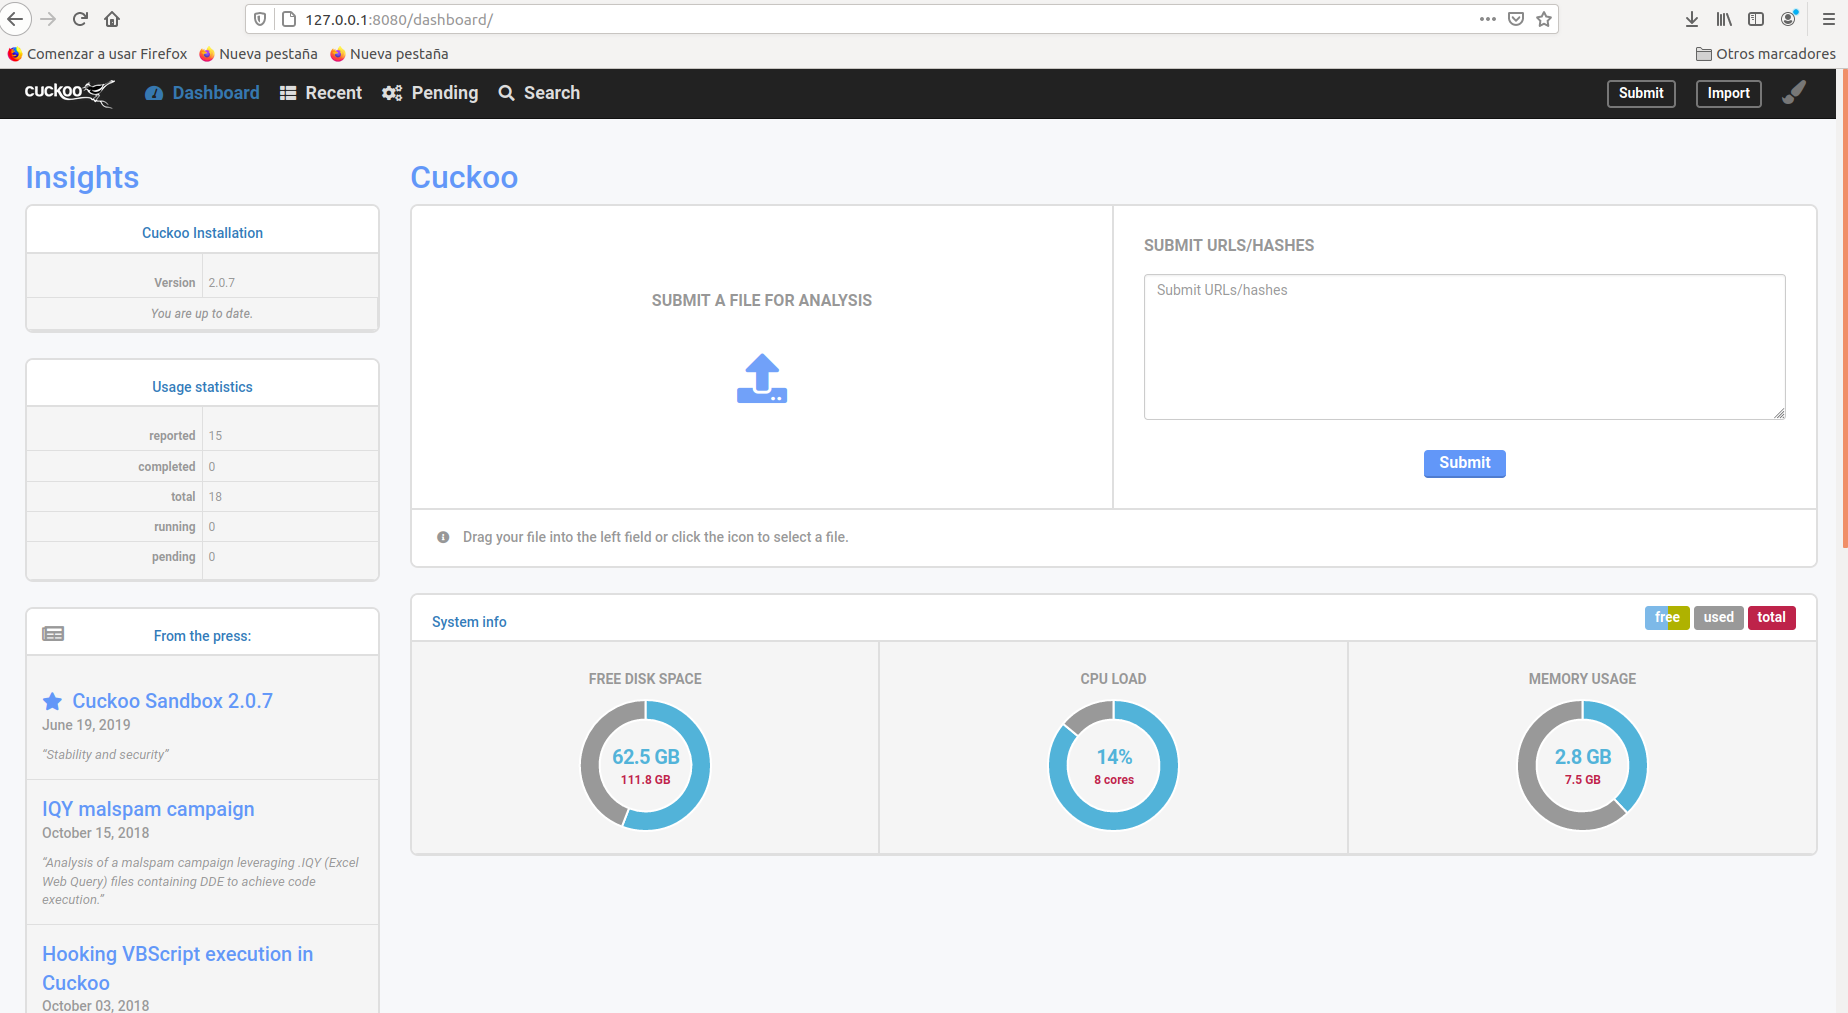
\includegraphics[width=0.9\linewidth]{images/principalcuckoo.png}
\end{center}
\caption{Pantalla principal Cuckoo Sandbox}
\label{fig:DashboardCuckoo}
\end{figure}

Al subir un archivo de malware para analizar, es posible configurar las opciones del análisis para todas las muestras o personalizar cada una. Entre las opciones, la que más interesa es la de "Internet" dentro de "Network Routing", para permitir al proceso acceder a conexión a Internet durante la ejecución. En la Figura \ref{fig:confAnalisis} se pueden observar distintas opciones de configuración.

\begin{figure}[h!]
\begin{center}
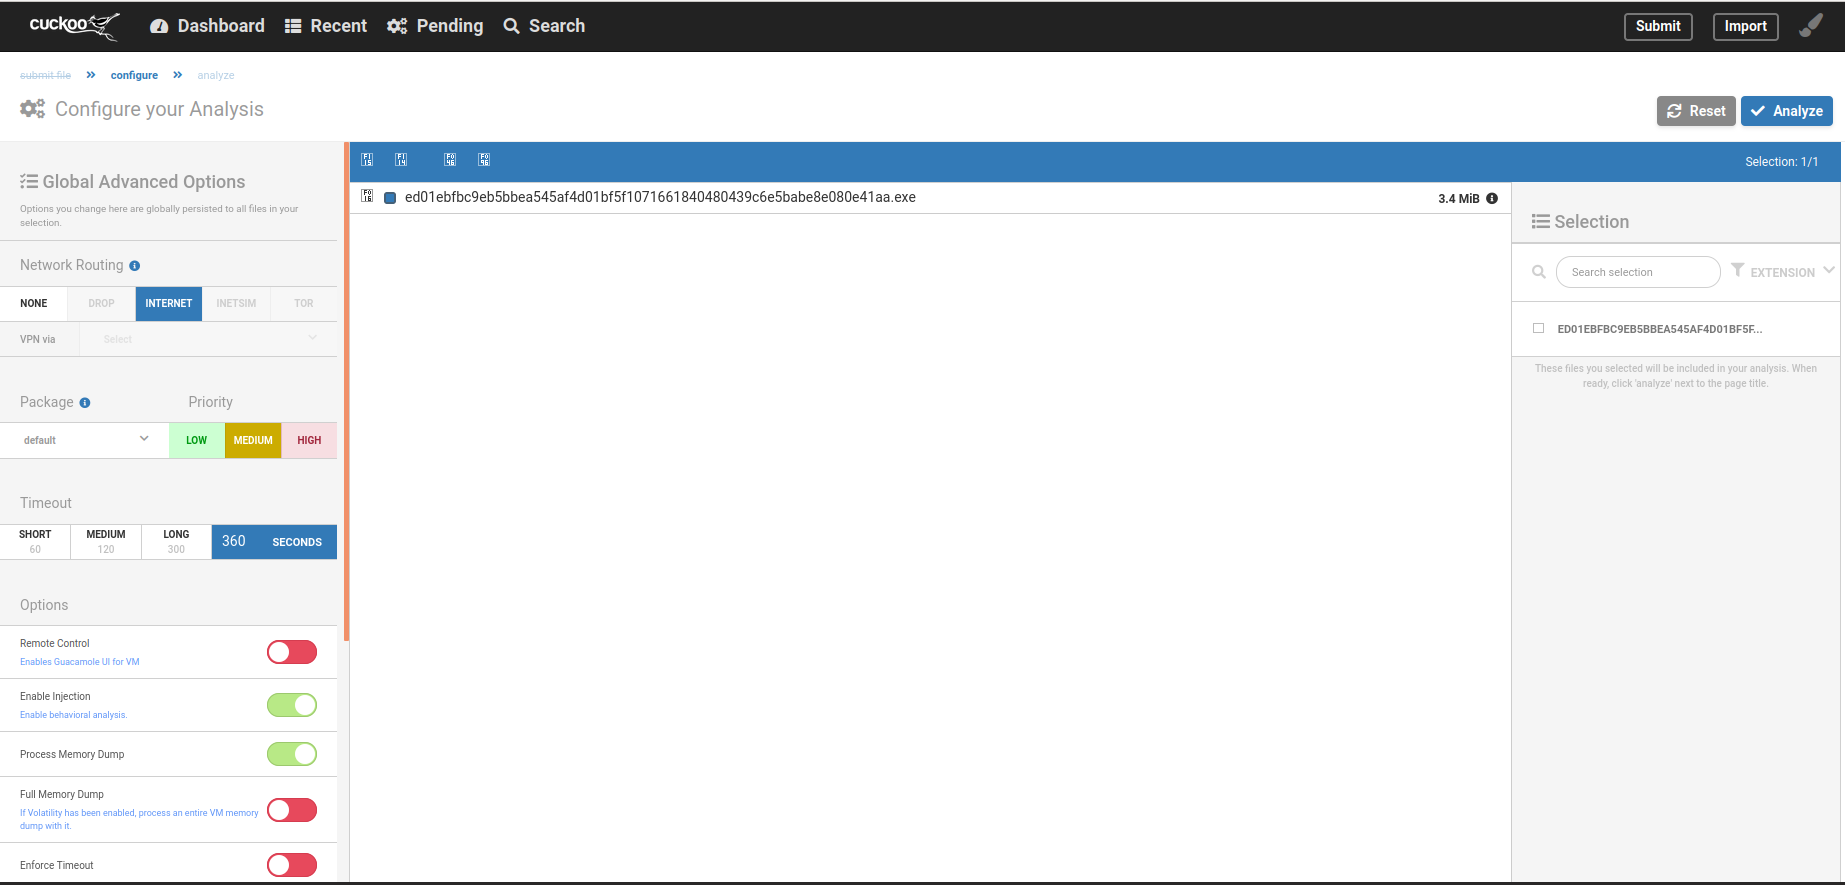
\includegraphics[width=0.9\linewidth]{images/configuracionanalisis.png}
\end{center}
\caption{Configuración del análisis}
\label{fig:confAnalisis}
\end{figure}

Después de configurar las opciones, pulsando en "Analyze" comenzará el análisis y se podrá observar cómo se abre la máquina virtual de Windows 7 y comienza la ejecución, viendo en todo momento qué va ocurriendo. Si se decide cambiar la configuración de Cuckoo para que no aparezcan las máquinas virtuales, no se podrá observer el comportamiento en directo de la muestra pero al haber instalado la herramienta "pillow" en las máquinas virtuales, se realizarán capturas de pantalla de lo que está ocurriendo.

En las Figuras \ref{fig:avisomalware} y \ref{fig:pagorescate}, se pueden observar capturas de pantalla realizadas durante el proceso de análisis que muestran un aviso de equipo infectado y una pantalla de instrucciones para el pago del rescate por la encriptación.

\begin{figure}[h!]
\begin{center}
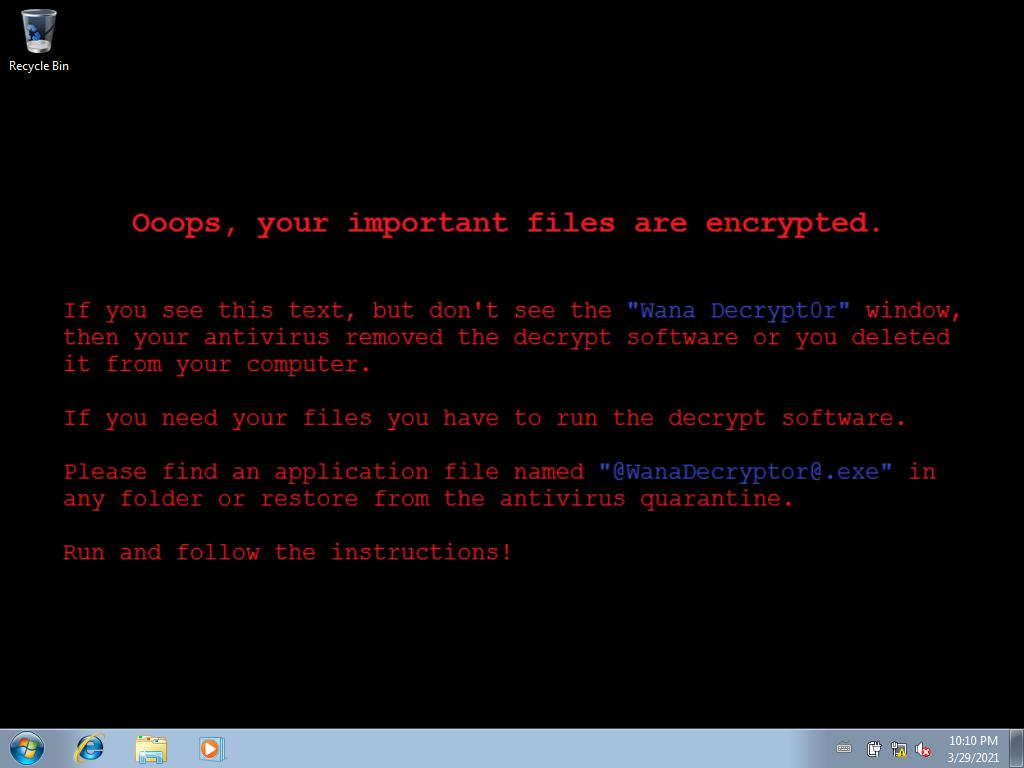
\includegraphics[width=0.72\linewidth]{images/wannacry1.jpg}
\end{center}
\caption{Aviso de malware}
\label{fig:avisomalware}
\end{figure}

\begin{figure}[h!]
\begin{center}
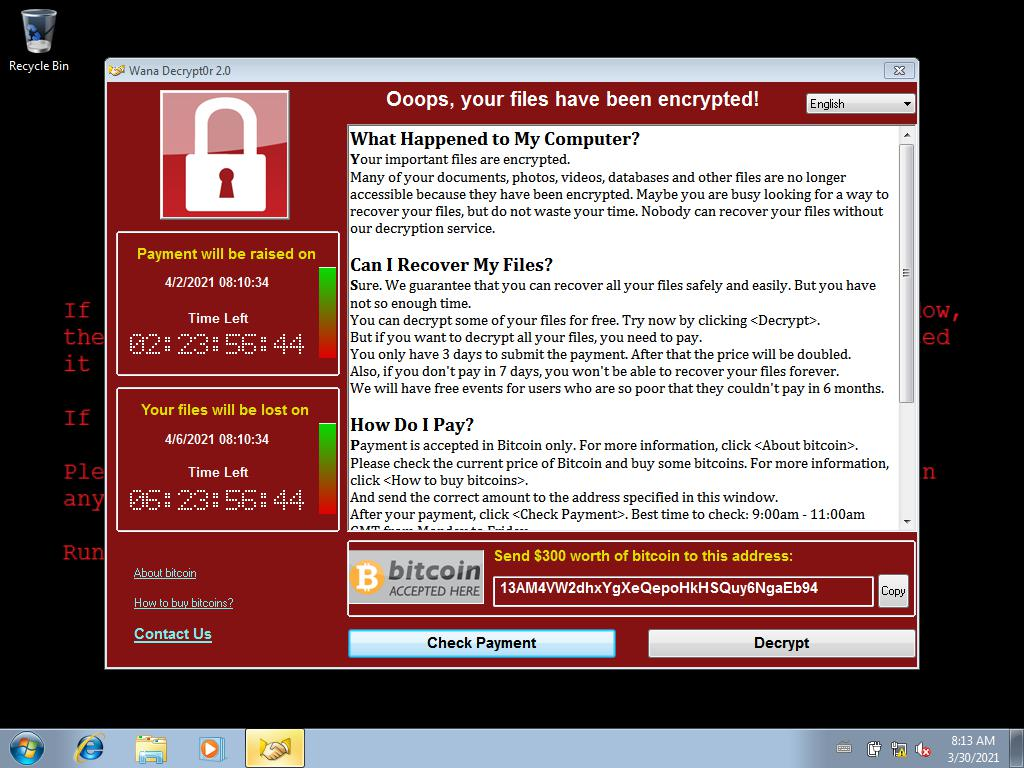
\includegraphics[width=0.72\linewidth]{images/wannacry2.jpg}
\end{center}
\caption{Pantalla de pago del rescate}
\label{fig:pagorescate}
\end{figure}

Al terminar, la máquina virtual se cerrará y en el navegador se podrán visualizar los resultados del análisis, con la puntuación obtenida, detalles técnicos sobre la muestra, capturas de pantalla, información sobre los eventos y su peligrosidad y un menú lateral para acceder a distintas características, entre otras cosas, tal y como se muestra en las Figuras \ref{fig:resulanalisis1} y \ref{fig:resulanalisis2}.

\begin{figure}[h!]
\begin{center}
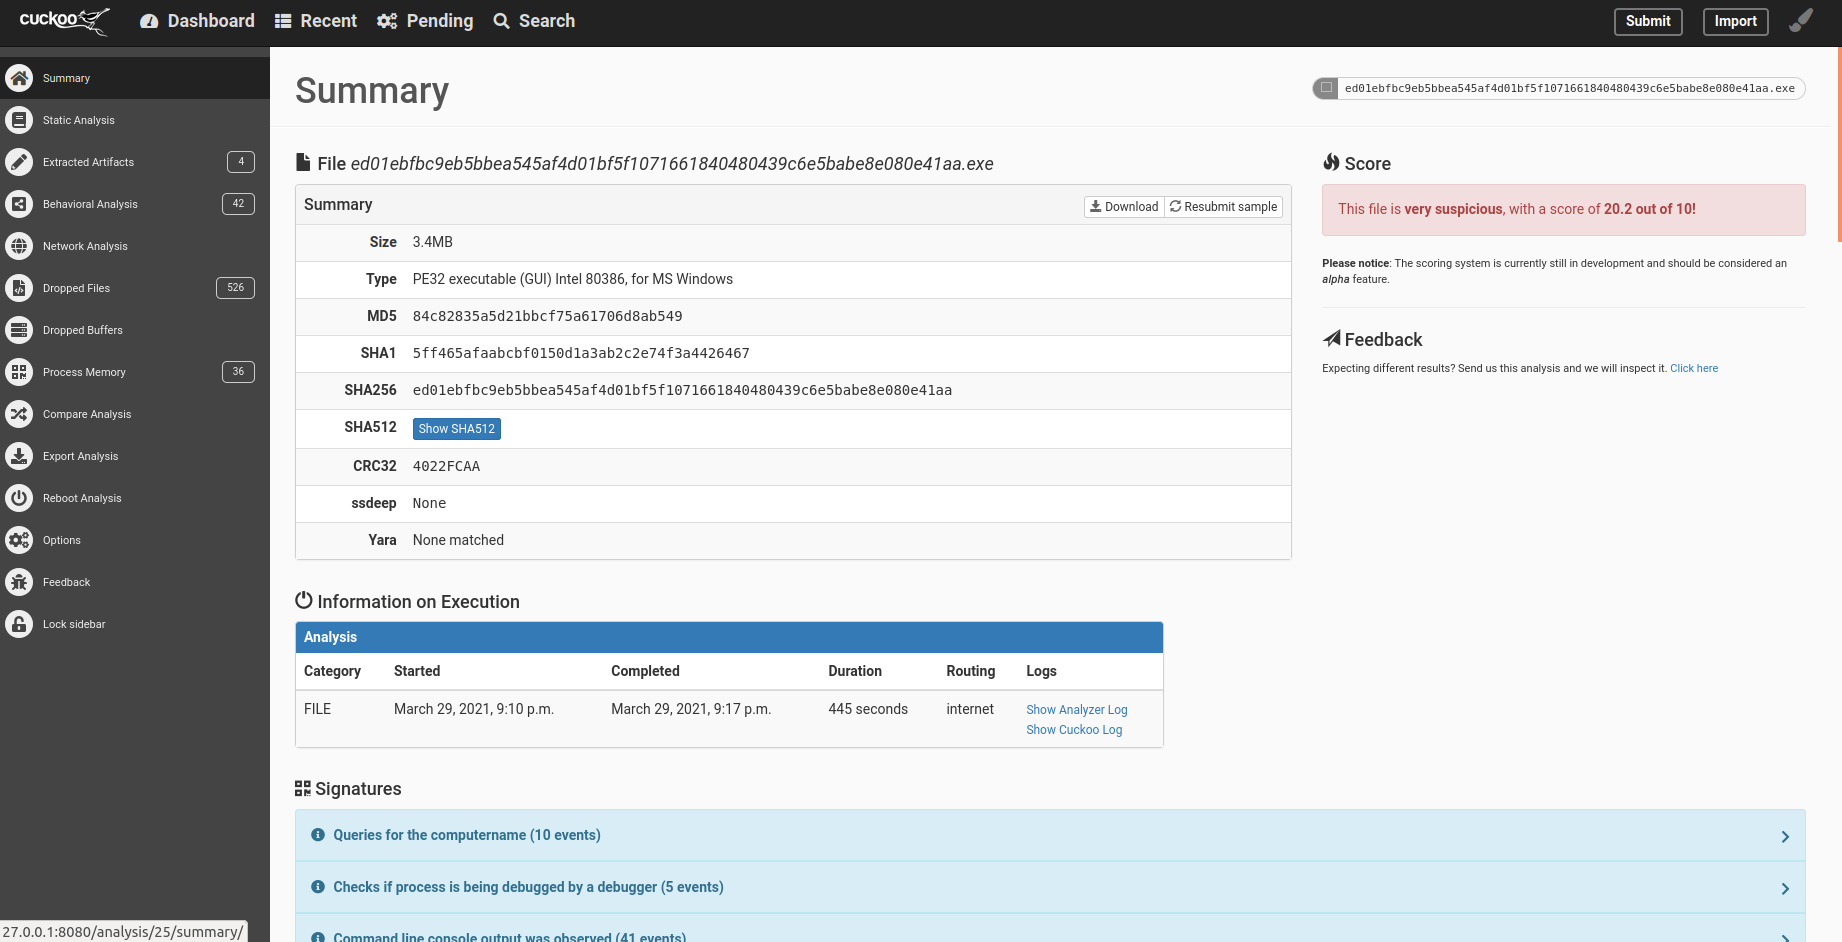
\includegraphics[width=0.9\linewidth]{images/resultadosanalisis1.png}
\end{center}
\caption{Resultados de análisis 1}
\label{fig:resulanalisis1}
\end{figure}

\begin{figure}[h!]
\begin{center}
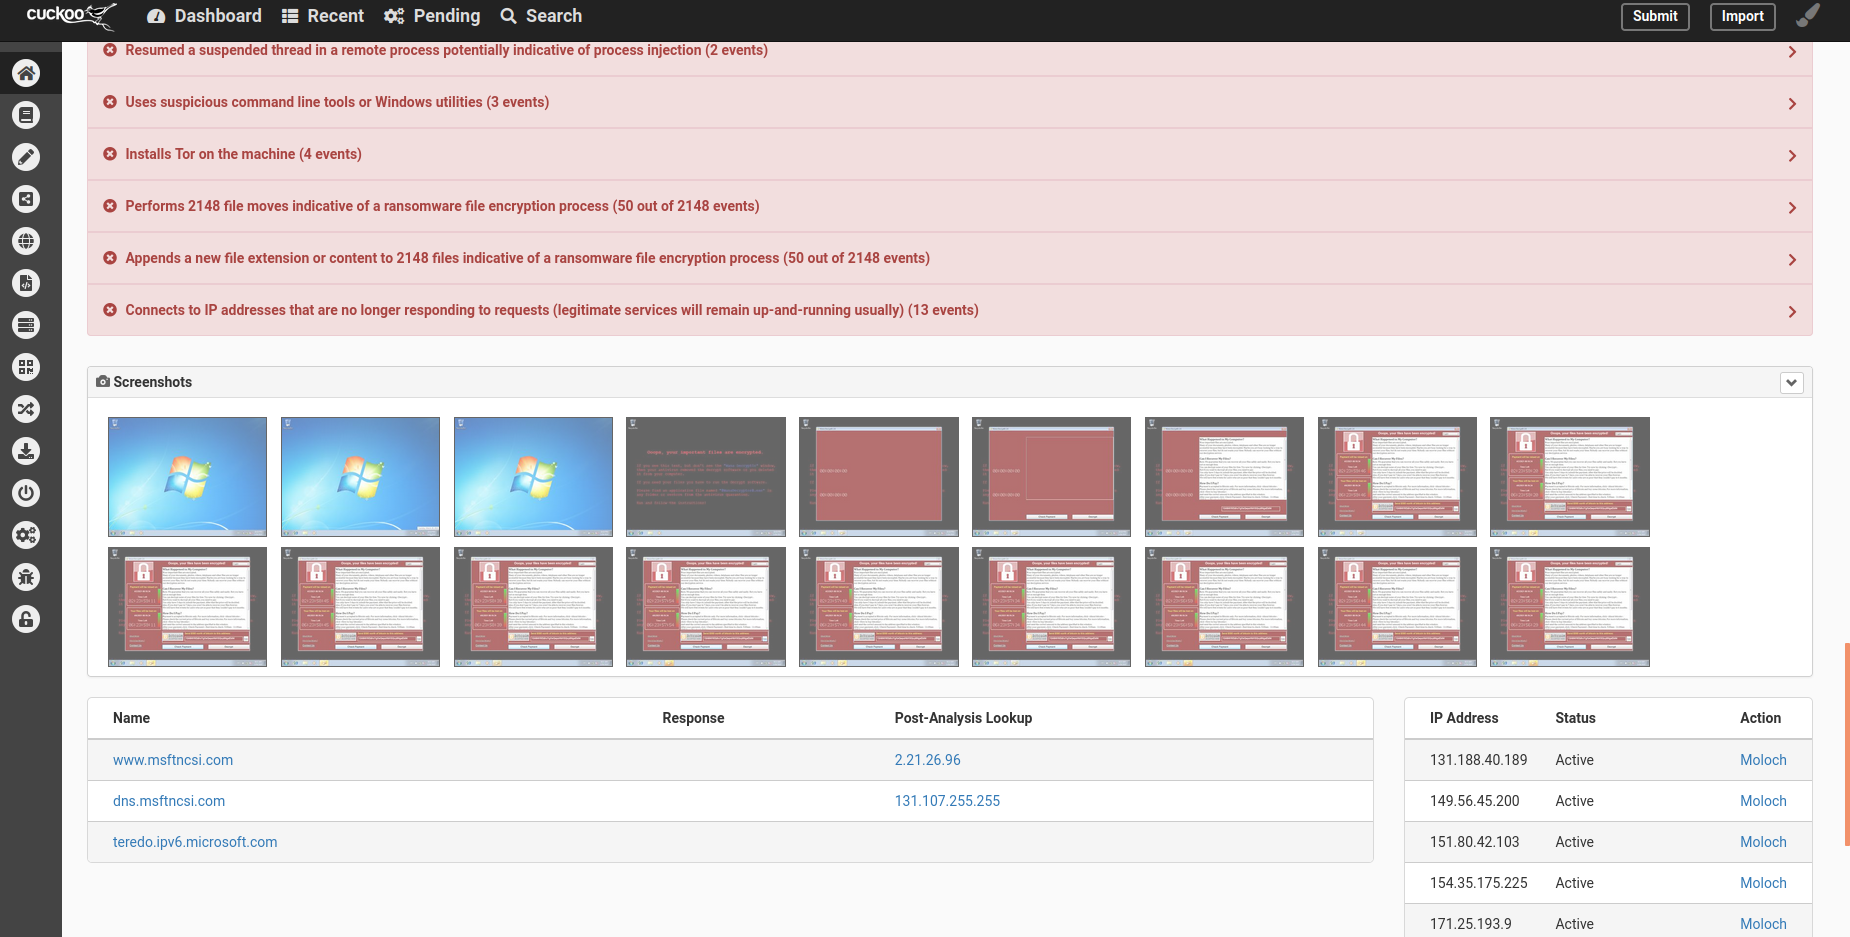
\includegraphics[width=0.9\linewidth]{images/resultadosanalisis2.png}
\end{center}
\caption{Resultados de análisis 2}
\label{fig:resulanalisis2}
\end{figure}

Toda esta información que se encuentra en la interfaz web, estará también en la carpeta ``storage'' dentro del directorio principal de trabajo de Cuckoo, organizada por carpetas para cada muestra, y repartida en sus correspondientes archivos de extensión ``.log'', ``.json'', ``.pcap''...
